\chapter{関連研究}

\section{行動情報から心的状態を推定する研究}
\par
行動情報から心的状態を推定する研究として,人間の心的状態理論Theory of Mind (ToM) \cite{子安増生1997心の理論}をベイズ推定を用いてモデル化するBayesian Theory of Mind (BToM) \cite{baker2011bayesian}が存在する.BToMは,環境の状態や人間の心的状態を部分的に観測可能なマルコフ決定過程\cite{alma9926438829904034}として表し,環境における人間の意思決定をベイズ推定に適用することで,環境中で人間が観測できていない部分についての信念と欲求を推定する.図\ref{fig:btom}に,BToMにおけるベイズ推定を表現するベイジアンネットワーク\cite{alma9926301926204034}を示す.$s_t$および$a_t$は観測値,$o_t$,$b_t$および$d$は確率変数として扱う.
\begin{figure}[htbp]
  \begin{center}
    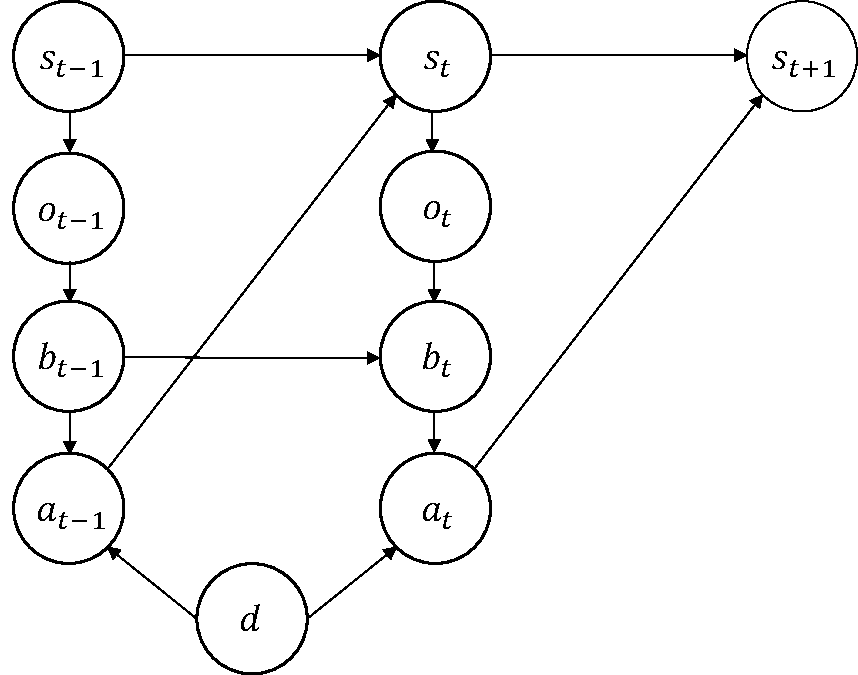
\includegraphics[scale=0.7]{./btom.pdf}
    \caption{BToMにおけるベイズ推定を表現するベイジアンネットワーク}
    \label{fig:btom}
  \end{center}
\end{figure}
BToMにおけるベイズ推定では,時刻$t$における環境の状態$s_{t}$を基に人間の観測状況$o_{t}$が計算される.また,$o_{t}$を基に人間の信念$b_{t}$が計算され,$b_{t}$と人間の欲求$d$から人間の行動$a_{t}$が計算される.$a_{t}$が起こることにより,環境の状態は$s_{t+1}$に変化し,人間の観測状況,信念および行動が再び計算される.BToMでは,時刻$1$から時刻$t$までの環境の状態遷移$s_{1:t}$と時刻$1$から時刻$t-1$までの人間の行動履歴$a_{1:t-1}$から計算される信念$b_t$と欲求$d$の確率$P(b_t,d|s_{1:t},a_{1:t-1})$を解くことを目的としている.ベイズの定理\cite{ベイズ}と図\ref{fig:btom}における変数間の独立性\cite{ベイズ}より,式(\ref{btom})が成り立つ.
\begin{equation}
  \begin{split}
  \label{btom}
  P(b_t,d|s_{1:t},a_{1:t-1}) &\propto P(b_t,d,s_{1:t},a_{1:t-1})\\
  &= \sum_{b_{t-1},o_t}P(b_t,d,s_{1:t},a_{1:t-1},b_{t-1},o_t)\\
  &= \sum_{b_{t-1},o_t}P(b_t|d,s_{1:t},a_{1:t-1},b_{t-1},o_t)\cdot P(d,s_{1:t},a_{1:t-1},b_{t-1},o_t)\\
  &= \sum_{b_{t-1},o_t}P(b_t|b_{t-1},o_t)\cdot P(o_t|d,s_{1:t},a_{1:t-1},b_{t-1})\cdot P(d,s_{1:t},a_{1:t-1},b_{t-1})\\
  &= \sum_{b_{t-1},o_t}P(b_t|b_{t-1},o_t)\cdot P(o_t|s_t)\cdot P(s_t|s_{t-1},a_{t-1})\\
  &\hspace{3cm} \cdot P(a_{t-1}|b_{t-1},d)\cdot P(b_{t-1},d,s_{1:t-1},a_{1:t-2})\\
  &\propto \sum_{b_{t-1},o_t}P(b_t|b_{t-1},o_t)\cdot P(o_t|s_t)\cdot P(s_t|s_{t-1},a_{t-1})\\
  &\hspace{3cm} \cdot P(a_{t-1}|b_{t-1},d)\cdot P(b_{t-1},d|s_{1:t-1},a_{1:t-2})\\
  \end{split}
\end{equation}
ここで,$P(b_t|b_{t-1},o_t)$は人間の観測$o_t$によって信念$b_t$が更新される確率,$P(o_t|s_t)$は環境の状態$s_t$において人間が観測状況$o_t$を得る確率,$P(s_t|s_{t-1},a_{t-1})$は環境の状態$s_{t-1}$において,人間が行動$a_{t-1}$を起こした時に環境の状態が$s_t$になる確率,$P(a_{t-1}|b_{t-1},d)$は人間が信念$b_{t-1}$,欲求$d$を持つ時に行動$a_{t-1}$を起こす確率,$P(b_{t-1},d|s_{1:t-1},a_{1:t-2})$は時刻$t-1$におけるBToMの出力である.式(\ref{btom})より,$P(b_t,d|s_{1:t},a_{1:t-1})$は初期値$P(b_1,d|s_1,a_0)$を決めて順次更新する計算により求めることができる.
% また,$P(b_t,d|s_{1:t},a_{1:t-1})$は$P(b_t|b_{t-1},o_t)$,$P(o_t|s_t)$,$P(s_t|s_{t-1},a_{t-1})$および$P(a_{t-1}|b_{t-1},d)$の乗算として表すことができる.


\par
行動情報から心的状態を推定する他の研究には,自動車の運転行動から心的状態を推定する研究 \cite{darwish2020learning}も存在する.自動車の運転では,運転者の心的状態によりスピードや前方車との車間距離が異なる.また,天候や時間によって運転者が選択する行動は変化する.運転者がどのような行動を起こすことを意図しているかを推定するために,交通状況を部分的に観測可能なマルコフ決定過程として表し,運転者の心的状態をBToMを用いてモデル化している.その結果,自動運転において運転者の意図に沿った動作の実現を手助けする.

\par
また,作業用ロボットに行動情報と心的状態の関係を適用した研究 \cite{inbook}も存在する.人間の作業員のアシスタントとして,人間の意図を推定することができるロボットを導入することで,効率的かつ安全な作業を行うことを目的としている.この研究における意図推定においては,人間の心的状態の移り変わりも考慮している.

\section{言語情報から心的状態を推定する研究}
\par
言語情報から心的状態を推定する研究として,発話から対話システムの信念や欲求,意図を推定する研究 \cite{高橋拓誠2015bdi}がある.意図を持った対話を行う対話システムの実現のために,信念と欲求を推定し,意図が生成される.この研究では,Beliefモジュール,Desireモジュール,Intentionモジュールから構成されるモデルを用いて意図を推定する.最初に,Beliefモジュールは発話から事象を抽出し,信念として捉える.Desireモジュールは,Beliefモジュールにおいて捉えられた信念を基に欲求の候補を複数生成する.また,生成された欲求の候補に対し,情緒生起手法 \cite{2002}を適用し,それぞれの尤度を算出し,最も尤度が高いものを欲求とする.Intentionモジュールは,Desireモジュールにおいて選択された欲求を基に意図生成を行う.

\par
また,検索精度向上のために言語情報と心的状態の関係を適用する研究 \cite{10.1007/978-3-642-02481-8_4}も存在する.ユーザの心的状態を考慮し,それを検索に反映することで,よりユーザが欲する情報を提供することに取り組んでいる.

\section{SCAIN}
対話において相手の心的状態を推定するためには,対話の文脈と心的状態の推定の相互依存性を解決することが必要である.対話において,文脈が相手の心的状態の推定に影響を与えたり,相手の心的状態により文脈が変わることがある.対話における文脈と単語の解釈の相互依存性を逐次的に解決する研究として,SCAIN \cite{takimoto2020slaminspired}が存在する.対話において,文脈により単語の解釈が変わったり,単語の解釈によって文脈が変わることがあり,対話の文脈と単語の解釈には相互依存性があるといえる.SCAINでは,対話履歴を対話の文脈として捉え,対話の文脈の推定と単語の解釈を並行して行うことで,文脈と単語の解釈の相互依存性の解決に取り組んでいる.

\section{関連研究における心的状態推定の問題点}
\par
心的状態を推定する関連研究における問題は,行動情報と発話情報の一方のみを推定に活用している点である.人間同士の対話では,行動によって発話の解釈が変わったり,発話によって行動の解釈が変わることは少なくない.対話システムと人間との対話においても,行動によって発話の解釈を変えたり,発話によって行動の解釈を変えることが重要である.そのため行動情報と発話情報の両方を活用した心的状態の推定が必要である.心的状態を推定する関連研究は,いずれも行動情報もしくは発話情報を含む言語情報の一方のみを心的状態の推定に活用したものである.これらの推定は,行動情報のみを観測できる場合や発話情報のみを観測できる場合には有効であるが,行動情報と発話情報の両方を観測できる場合においては不十分である.行動情報と発話情報の一方のみの単一情報による心的状態の推定では,行動による発話の解釈の変化や発話による行動の解釈の変化を捉えることができず,行動情報と発話情報の相互作用を考慮して心的状態を推定することができない.

% \par
% またSCAINにおける問題点は,対話の文脈と単語の解釈の相互依存性を解決する際に,文脈として対話履歴のみを採用している点である.実世界では,文脈として捉えることができるものは対話履歴だけではない.対話相手の行動から得られる情報も単語の解釈において重要な文脈として扱うことができる.対話の文脈と単語の解釈の相互依存性を解決するにあたり行動情報が有益である際に,SCAINの有効性が低下してしまうことが考えられる.

\section{MIoM SCAINと関連研究との相違点}
\par
MIoM SCAINと関連研究との相違点は,行動情報と発話情報の両方を活用したマルチモーダルな心的状態推定を行う点である.MIoM SCAINは,行動情報と発話情報の両方を活用して心的状態を推定する際に,SCAINにおける文脈と単語解釈の相互依存性の解決のように行動情報と発話情報の相互依存性を扱うことで,発話による行動の解釈の変化や行動による発話の解釈の変化を捉え,行動情報と発話情報の相互作用を考慮した推定が可能となる.MIoM SCAINは,関連研究における問題点を解消するシステムとなっている.
